\documentclass[a4paper,11pt]{article}


%\usepackage{macros}
\usepackage{jheppub}

\usepackage[T1]{fontenc}
\usepackage{lmodern}
\usepackage{amsmath}
\usepackage{amsfonts}
\usepackage{amssymb}
\usepackage{amsthm}
\usepackage{mathrsfs}
\usepackage{physics}
\usepackage{graphicx}
\usepackage{subcaption}
\usepackage{enumitem}
\usepackage{framed,float}
\usepackage{booktabs}
\usepackage{array}
\usepackage{soul}
\usepackage{multirow}
\usepackage{comment}
\usepackage{braket}
\usepackage{todonotes}
\usepackage{youngtab}
\usepackage{tikz}
\usetikzlibrary{calc,arrows,decorations.markings}

%\usepackage{geometry}

\usepackage{color}


\title{Helicity Selection Rules in Double Copy Formulae for Scattering Amplitudes}
\author{Author: Qingjie Yuan,$\qquad\qquad\qquad\qquad\qquad\qquad$}
\author{Supervisor: Oliver Schlotterer}
\affiliation{Department of Physics and Astronomy, Uppsala University, \\Box 516, 75120 Uppsala, Sweden}
\emailAdd{qingjie.yuan.9461@uu.student.se}

\abstract{This report reviews the double copy structure of scattering amplitudes, focusing on its underlying algebra and application to selection rules.
We first discuss how color-kinematic duality naturally emerges in self-dual Yang-Mills theory through the construction of kinematic numerators satisfying so-called kinematic algebra. 
Then we turn to Born-Infeld theory and examine how its helicity selection rules arise from the double copy perspective. In particular, we show that the vanishing tree-level four-dimensional Born-Infeld amplitudes 
can result from nontrivial cancellation between nonzero Yang-Mills and nonlinear sigma model amplitudes via KLT double copy. Finally, we comment on possible generalizations and open problems for future research.}
\begin{document}
\newcommand{\sket}[1]{|#1]}
\newcommand{\sbra}[1]{[#1|}
\newcommand{\ads}[3]{\langle #1|#2|#3]}
\newcommand{\sda}[3]{[#1|#2|#3\rangle}
\renewcommand{\braket}[1]{\langle #1 \rangle}
\newcommand{\Xij}[2]{\braket{\eta #1}[#1 #2]\braket{#2 \eta}}

\newcommand{\etal}[1]{\braket{\eta #1}}
\newcommand{\etar}[1]{\braket{#1 \eta}}


\maketitle
\tableofcontents

\allowdisplaybreaks
%%%%%%%%%%%%
\section{Introduction}
Recent years have seen remarkable progress in our understanding of scattering amplitudes, particularly in gauge theory and gravity.
One of the most striking developments is the discovery of the double copy structure, which relates amplitudes in gravity to those in gauge theory.
The idea can be traced back to the Kawai-Lewellen-Tye (KLT) relations in string theory \cite{Kawai:1985xq}, which express closed string amplitudes as sums over products of open string amplitudes.
In the field theory limit, these relations survive as a prescription for constructing gravity amplitudes from gauge-theory ones. The KLT relation provides both conceptual insight
and concrete tools in the study of scattering amplitudes. This connection not only offers computational advantages,
but also hints at a deeper unity underlying different physical theories. However, this relation is largely confined to tree-level (or, at best, to certain one-loop cases \cite{He:2016mzd}).\par

Bern, Carrasco, and Johansson (BCJ) introduced a novel perspective of double copy based on the concept of color-kinematics (CK) duality \cite{Bern:2008qj,Bern:2010ue}.
This duality is not only formulated at tree level, also manifests in multi-loop amplitudes.
In theories where CK duality holds, the scattering amplitudes can be rearranged so that kinematic numerators satisfy the same algebraic relation, like Jacobi identities, 
as their color numerators. Remarkably, by replacing color factors with dual kinematic factors, we can convert gauge-theory scattering amplitudes to gravity ones. 
More importantly, CK duality and double copy are not confined to gauge and gravity theories, 
it has been identified in several other theoretical frameworks. Many theories are connected by double copy relations and other structural links, 
form what is now often referred to as a web of theories,
for a review, see \cite{Bern:2019prr,Bern:2022wqg,Adamo:2022dcm}, which may point towards deeper algebraic structures underlying scattering amplitudes.
This process can be simply described as
\begin{equation}
    \begin{split}
    \mathcal{A}^{\text{theory L}}\sim& (\text{color})\times (\text{kinematic L}),\qquad \mathcal{A}^{\text{theory R}}\sim (\text{color})\times (\text{kinematic R})\\
        &\mathcal{M}^{\text{theory L}\otimes\text{R}}\sim (\text{kinematic L})\times (\text{kinematic R})
    \end{split}
\end{equation}
From this schematic rule, we can easily see why it is called the double copy relation.\par

We begin by reviewing the spinor-helicity language \cite{Dixon:1996wi,Elvang:2015rqa}, in which the amplitudes in 4-dimensional Yang-Mills theory and its self-dual sector can be expressed in a simple and elegant way. 
We then examine how CK duality emerges in the self-dual Yang-Mills (SDYM) theory \cite{Monteiro:2011pc,Boels:2013bi,He:2015wgf} and in the non-linear sigma model (NLSM) \cite{Du:2016tbc,Carrasco:2016ldy,Carrasco:2016ygv,Cheung:2016prv}, 
a low-energy effective theory describing the dynamics of Goldstone bosons, with explicit numerator construction in the references \cite{Du:2016tbc,Carrasco:2016ldy,Carrasco:2016ygv,Cheung:2016prv}.
Although the NLSM is not a gauge theory, its Goldstone bosons are $U(N)$ Lie-algebra-valued, and some theoretical evidence suggests that 
amplitudes in Born-Infeld (BI) theory \cite{Born:1934gh,Tseytlin:1999dj} can be constructed as a double copy of Yang-Mills and NLSM amplitudes \cite{Cachazo:2014xea,Cachazo:2015ksa}.
This is one of the nontrivial extensions of CK duality and double copy beyond traditional gauge frameworks. 
In this work, we explore how BI amplitudes can be built from numerators in YM and NLSM that satisfy appropriate algebraic identities, 
and we investigate how this construction captures the helicity selection rules of amplitudes in BI theory. 
Although the double copy itself is not restricted to specific spacetime dimensions, we will focus on four-dimensional case.
Helicity refers to the projection of a massless particle's spin along its momentum direction, taking value $\pm 1$ for spin-$1$ particles. 
The helicity selection rule here states that BI amplitudes are only non-zero when the external states consist of equal numbers of positive and negative helicity particles.\par
The report is organized as follows. Section 2 is a review of spinor-helicity formalism and amplitudes in Yang-Mills theory, with its MHV amplitudes and self-dual sector given as examples. 
In section 3, we study CK duality in SDYM and NLSM, and describe how their structure supports a double copy framework. Section 4 focuses on BI theory, examining its amplitude properties and selection rules, 
and providing explicit calculations at four and six points partially. We conclude in section 5 with a discussion of open questions.
%%%%%%%%%%%%
\section{Spinor-Helicity formalism}
\subsection{Spinor-helicity for four-dimensional massless particles}
The spinor-helicity formalism provides an efficient and elegant framework for expressing scattering amplitudes, 
particularly in four-dimensional massless theories. 
Since this paper focuses on four-dimensional gauge and scalar theories with massless external states, 
all amplitudes discussed will be expressed in the spinor-helicity language. In this subsection, 
we briefly review this formalism and establish the conventions used throughout the paper.\par

In this formalism \cite{Dixon:1996wi}, an on-shell momentum $k^2=0$ is expressed in terms of two two-component commuting spinors, $\lambda$ and $\tilde{\lambda}$,
\begin{equation}
    k_{\alpha \dot{\alpha}}\equiv k_{\mu}\sigma^{\mu}_{\alpha \dot{\alpha} }=\lambda_\alpha \tilde{\lambda}_{\dot{\alpha}},
\end{equation}
where $\sigma^\mu=(1_{2\times 2},\sigma^i)$, the $\sigma^i$ are the Pauli matrices and the range of indices are $\mu=0,1,2,3$ and $\alpha=1,2;\, \dot\alpha=\dot{1},\dot{2}$. It is customary to denote these spinors using angle and aquare brackets,
\begin{equation}
    \ket{i}\equiv \begin{pmatrix}
        \lambda_1^{(i)}\\
        \lambda_2^{(i)}
    \end{pmatrix},\qquad \sket{i}\equiv \begin{pmatrix}
    -\tilde{\lambda}^{(i){\dot{1}}}\\
    -\tilde{\lambda}^{(i){\dot{2}}}
    \end{pmatrix}.
\end{equation}
Raising and lowering spinor indices is performed by the anti-symmetric Levi-Civita tensor $\epsilon^{\alpha \beta}$ and $\epsilon^{\dot{\alpha}\dot{\beta}}$,
\begin{equation}
    \lambda^\alpha=\epsilon^{\alpha \beta}\lambda_\beta,\quad \tilde{\lambda}^{\dot{\alpha}}=\epsilon^{\dot{\alpha}\dot{\beta}}\tilde{\lambda}_{\dot \beta},
    \quad \lambda_\alpha=\epsilon_{\alpha \beta}\lambda^\beta,\quad \tilde{\lambda}_{\dot{\alpha}}=\epsilon_{\dot{\alpha}\dot{\beta}}\tilde{\lambda}^{\dot \beta}.
\end{equation}
And the dual brackets,
    \begin{equation}
        \bra{i}\equiv \big(-\lambda^{(i)1},-\lambda^{(i)2}\big)
        ,\qquad \sbra{i}\equiv 
        \big(\tilde{\lambda}_{\dot{1}}^{(i)},
        \tilde{\lambda}_{\dot{2}}^{(i)}\big).
    \end{equation}
With this notation, the momentum $k_i$ becomes,
\begin{equation}
    k_i=\begin{pmatrix}
        \lambda_1^{(i)}\tilde{\lambda}_{\dot{1}}^{(i)}&\lambda_1^{(i)}\tilde{\lambda}_{\dot{2}}^{(i)}\\
        \lambda_2^{(i)}\tilde{\lambda}_{\dot{1}}^{(i)}&\lambda_2^{(i)}\tilde{\lambda}_{\dot{2}}^{(i)}
    \end{pmatrix}=\ket{i}\sbra{i}
\end{equation}
The spinor inner products for two on-shell momentum $k_i,k_j$ are defined as (actually it has been defined from the dual brackets),
\begin{equation}
    \braket{ij}=-\epsilon^{\beta \alpha}\lambda^{(i)}_{\alpha}\lambda^{(j)}_{\beta}=\epsilon^{\alpha\beta}\lambda^{(i)}_{\alpha}\lambda^{(j)}_{\beta},
\end{equation}
and
\begin{equation}
    [ij]=-\epsilon^{\dot{\alpha}\dot{\beta}}\tilde{\lambda}^{(i)}_{\dot{\alpha}}\tilde{\lambda}^{(j)}_{\dot{\beta}}.
\end{equation}
we can easily check they are both antisymmetric, $\braket{ij}=-\braket{ji}$ and $[ij]=-[ji]$. A useful result is,
\begin{equation}
    \begin{split}
        \braket{ij}[ji]=&\epsilon^{\alpha\beta}\lambda^{(i)}_{\alpha}\lambda^{(j)}_{\beta}\epsilon^{\dot{\alpha}\dot{\beta}}\tilde{\lambda}^{(i)}_{\dot{\alpha}}\tilde{\lambda}^{(j)}_{\dot{\beta}}\\
        =& k_i^\mu k_j^\nu \epsilon^{\alpha\beta}\epsilon^{\dot{\alpha}\dot{\beta}}\sigma^{\mu}_{\alpha\dot{\alpha}}\sigma^{\nu}_{\beta\dot \beta}\\
        =&2k_i\cdot k_j=s_{ij}.
    \end{split}
\end{equation}
In the last line, $\epsilon^{\alpha\beta}\epsilon^{\dot{\alpha}\dot{\beta}}\sigma^{\mu}_{\alpha\dot{\alpha}}\sigma^{\nu}_{\beta\dot \beta}=2\eta^{\mu \nu}$ is used. This identity is widely used in expressing Mandelstam variables. 
For a list $X$ of particle labels, $s_X=(k_{X_1}+k_{X_2}+\cdots k_{X_{|X|}})^2$. 
The notation $\braket{ij}$ can be extend to,
\begin{equation}
    \ads{i}{j}{l}=-\lambda_{\alpha}^{(i)}\epsilon^{\alpha\beta}k_{\beta\dot{\alpha}}^{(j)}\epsilon^{\dot{\alpha}\dot{\beta}}\lambda_{\dot{\beta}}^{(l)}=-\sda{l}{j}{i},
\end{equation}
\begin{equation}
    \braket{i|jl|r}=\lambda_{\alpha}^{(i)}\epsilon^{\alpha\beta}k_{\beta\dot{\alpha}}^{(j)}\epsilon^{\dot{\alpha}\dot{\beta}}k_{\gamma\dot{\beta}}^{(l)}\epsilon^{\gamma\delta}\lambda_{\delta}^{(r)}=-\braket{r|lj|i},
\end{equation}
\begin{equation}
    [i|jl|r]=\tilde{\lambda}_{\dot{\alpha}}^{(i)}\epsilon^{\dot{\alpha}\dot{\beta}}k_{\alpha\dot{\beta}}^{(j)}\epsilon^{\alpha\beta}k_{\beta\dot{\gamma}}^{(l)}\epsilon^{\dot{\gamma}\dot{\delta}}\tilde{\lambda}_{\dot{\delta}}^{(r)}=-[r|lj|i].
\end{equation}
Here momentum $k$ need not to be on-shell. And for on-shell momentum, we have,
\begin{equation}
    \braket{i|jl|r}=\braket{ij}[jl]\braket{lr},\quad [i|jl|r]=[ij]\braket{jl}[lr].
\end{equation}
Now I write down the Schouten identity. for angle brakets,
\begin{equation}\label{Schouten-a}
    \braket{ij}\braket{kl}+\braket{ik}\braket{lj}+\braket{il}\braket{jk}=0,
\end{equation}
and analogous identities hold for the square brackets and mixed brackets,
\begin{equation}
    [ij][kl]+[ik][lj]+[il][jk]=0,
\end{equation}
These identities are extremely useful in simplifying spinor expressions and will be frequently used to manipulate amplitude formulas in later sections.\par

%%%%
\subsection{Examples from Yang-Mills theory}
In the remainder of this paper, we will frequently work with four-dimensional Yang-Mills theory, 
which can also serve as a concrete example to familiarize us with spinor-helicity formalism. Here we mainly consider maximally helicity violating (MHV) amplitudes, 
which means two negative-helicity external states amplitudes, and the self-dual sector.\par

\subsubsection{MHV amplitudes}
We now begin to directly verify the three-point MHV amplitude using Feynman rules in the spinor-helicity formalism.
This serves as an explicit example that illustrates how the formalism efficiently encodes helicity structure and simplifies perturbative calculations.
The Yang-Mills Lagrangian in light-cone gauge \cite{Chalmers:1998jb},
\begin{equation}
    \mathcal{L}=\tr\left\{\frac{1}{2}\bar{A}\partial^2A-ig\left(\frac{\partial_w}{\partial_u}A\right)[A,\partial_u\bar{A}]-ig\left(\frac{\partial_{\bar{w}}}{\partial_u}\bar{A}\right)[\bar{A},\partial_uA]-g^2[A,\partial_u\bar{A}]\frac{1}{\partial_u^2}[\bar{A},\partial_uA]\right\}.
\end{equation}
The light-cone is defined by a null vector $\eta$. The field $A$ and $\bar{A}$ carry positive and negative helicities separately. The indices are from the coordinates,
\begin{equation}
    u=t-z,\quad v=t+z,\quad w=x+iy,\quad \bar{w}=x-iy.
\end{equation}
The light-cone condition is $A_u=0$. There are three distinct types of interaction vertices from this Lagrangian, 
the three-point vertices involving either two positive-helicity and one negative-helicity gluon, or two negative-helicity and one positive-helicity gluon; 
and a four-point vertex involving two gluons of each helicity.
In spinor-helicity formalism, with $i_\eta=2k_i\cdot \eta=\braket{\eta i}[i \eta]$, these vertices can be written compactly as \cite{Boels:2013bi},
\begin{equation}
    \begin{split}
    (i^{+},j^{+},l^{-})=&\frac{l_{\eta}}{i_{\eta}j_{\eta}}X_{i,j}f^{a_{i}a_{j}a_{l}},\quad\mathrm{with}\quad X_{i,j}\equiv\langle\eta|k_{i}k_{j}|\eta\rangle,\\
    (i^{-},j^{-},l^{+})=&\frac{l_{\eta}}{i_{\eta}j_{\eta}}\overline{X}_{i,j}f^{a_{i}a_{j}a_{i}},\quad\mathrm{with}\quad\overline{X}_{i,j}\equiv[\eta|k_{i}k_{j}|\eta],\\
    (i^{+},j^{+},l^{-},r^{-})=&i\bigg(\frac{i_{\eta}l_{\eta}+j_{\eta}r_{\eta}}{(i_{\eta}+r_{\eta})^{2}}f^{a_{i}a_{r}b}f^{ba_{j}a_{l}}+\frac{i_{\eta}r_{\eta}+j_{\eta}l_{\eta}}{(i_{\eta}+l_{\eta})^{2}}f^{a_{i}a_{l}b}f^{ba_{j}a_{r}}\bigg),
    \end{split}
\end{equation}
together with the propagator,
\begin{equation*}
    \quad i \delta^{a_i a_j}/k^2,
\end{equation*}
and external state factors,
\begin{equation}
    \hat{e}^{(+)}_i=\frac{[\eta i]}{\braket{\eta i}},\qquad \hat{e}^{(-)}_i=\frac{\braket{\eta i}}{[\eta i]},
\end{equation}
they define the complete set of Feynman rules in this gauge and formalism.\par
Here we write down some useful properties of $X_{i,j}$ from its definition.
The antisymmetry
\begin{equation}
    X_{i,j}=\langle\eta|k_{i}k_{j}|\eta\rangle=-\langle\eta|k_{j}k_{i}|\eta\rangle=-X_{j,i},
\end{equation}
leading $X_{i+j,j}=X_{i,j}$, and Jacobi-type identity,
\begin{equation}\label{X-relation}
    X_{i,j}X_{i+j,l}+X_{j,l}X_{j+l,i}+X_{l,i}X_{l+i,j}=0.
\end{equation}\par

Three-point MHV amplitudes from the above rules,
\begin{equation}
    A(1^-,2^-,3^+)=\hat{e}^{(-)}_1 \hat{e}^{(-)}_2 \hat{e}^{(+)}_3 \frac{3_{\eta}}{1_{\eta}2_{\eta}}\overline{X}_{1,2}=\frac{\braket{\eta 1}\braket{\eta 2}[\eta 3]^2\braket{\eta 3}[\eta 1][\eta 2]\braket{12}}{[\eta 1]^2[\eta 2]^2 \braket{\eta3}\braket{\eta 1}\braket{\eta 2}}=\frac{[\eta 3]^2 \braket{12}}{[\eta 1][\eta 2]}.
\end{equation}
We can prove,
\begin{equation}
    \frac{[\eta 3]}{[\eta 1]}=\frac{[\eta 3]\braket{32}}{[\eta 1]\braket{32}}=\frac{[\eta 3]\braket{32}}{[\eta 1]\braket{32}}=\frac{-\sda{\eta}{k_1+k_2}{2}}{[\eta 1]\braket{32}}=-\frac{[\eta 1]\braket{12}}{[\eta 1]\braket{32}}=\frac{\braket{12}}{\braket{23}},
\end{equation}
where the momentum conservation $k_1+k_2+k_3=0$ is used. And
\begin{equation}
    \frac{[\eta 3]}{[\eta 2]}=\frac{\braket{12}}{\braket{31}}.
\end{equation}
From this process, we can see why the amplitudes are independent of the reference spinor $\eta$. Now the amplitude becomes,
\begin{equation}
    A(1^-,2^-,3^+)=\frac{\braket{12}^3}{\braket{23}\braket{31}}.
\end{equation}
The result matches the below Parker-Taylor formula when $n=3$, which in general is presented as \cite{Parke:1986gb,Berends:1987me},
\begin{equation}\label{pt-formula}
    A(1^+,\dots,r^-,\dots,s^-,\dots,n^+)=\frac{\braket{rs}^4}{\braket{12}\braket{23}\cdots\braket{n1}}.
\end{equation}

\subsubsection{Self-dual sector}
Now we turn to the self-dual sector of Yang-Mills theory. The self-dual Yang-Mills equation in Minkowski spacetime is,
\begin{equation}
    F_{\mu \nu}=\frac{i}{2}\epsilon_{\mu \nu \rho \sigma}F^{\rho \sigma}.
\end{equation}
In this sector, only the $(+,+,-)$ vertices are present. The Feynman rules simplify considerably and can be written as,
\begin{equation}\label{sd-f}
(i^+,j^+,l^-)^{\text{s.d.}}=X_{i,j}f^{a_i a_j a_l},\qquad \text{external: } e^{(+)}=-\frac{1}{\braket{\eta i}^2}, \quad e^{(-)}_i=-\braket{\eta i}^2,
\end{equation}
where $\text{s.d.}$ means self-dual.\par
As a result, all contributing Feynman diagrams are constructed solely from this type of vertex. 
By simple counting, one sees that at tree level, only amplitudes with a single negative-helicity external gluon can receive contributions. 
Physically, the self-dual sector corresponds to a restriction in which only one helicity state is present, typically taken to be positive-helicity gluons.
As a result, any tree-level amplitude, which has at least one negative helicity external gluon, must vanish.
In SDYM, the structure of color-kinematic duality naturally emerges and will be discussed in the next section.\par


%%%%%%%%%%%%%%%
\section{Color-kinematic duality}
In this section, we begin by reviewing the general formulation of CK duality. 
We then explore its simple realization in the SDYM, where the duality is manifest in a particularly transparent way.
To illustrate the broader significance of CK duality beyond gauge theories, we further consider the example of the NLSM.
\subsection{Theoretical statement}
\subsubsection{Color-ordered partial amplitudes}
Before discussing CK duality and double copy, it is helpful to briefly recall the notion of color-ordered partial amplitudes in gauge theory. 
At tree level, gauge theory amplitudes can be decomposed as a sum over color structures multiplied by so-called color-ordered or partial amplitudes as,
\begin{equation}\label{DDM}
    \mathcal{A}_m^{\text{tree}}=g^{m-2}\sum_{\sigma \in S_{m-1}}A_m^{\text{tree}}(1,\sigma(2,3,\dots,m-1,m))\Tr(T^{a_1}T^{a_{\sigma(2)}}T^{a_{\sigma(3)}}\cdots T^{a_{\sigma(m)}}).
\end{equation}
where the sum runs over $(m-1)!$ permutations and $T^{a_i}$ is the gauge group generators. In the remainder of this section, we omit explicit labels for tree-level. Unless otherwise noted, all amplitudes are understood to be at tree level. 
This decompositions can also be expressed in the adjoint generator $(\tilde{f}^{b})_{ac}=\tilde{f}^{abc}\equiv i\sqrt{2}f^{abc}$, called the Del Duca-Dixon-Maltoni (DDM) color decompositions \cite{DelDuca:1999rs}, as,
\begin{equation}
    \mathcal{A}_m=g^{m-2}\sum_{\sigma \in S_{m-2}}A_m(1,\sigma(2,3,\dots,m-1),m)(\tilde{f}^{a_{\sigma(2)}}\tilde{f}^{a_{\sigma(3)}}\cdots \tilde{f}^{a_{\sigma(m-1)}})_{a_1a_m},
\end{equation}
where the sum is taken over permutations of $m-2$ labels, rather than $m-1$ as in earlier expressions. The redundancy is eliminated by the relations of partial amplitudes given later. 
These partial amplitudes are depending only on the kinematic data (momentum and polarization), thus sometimes also called color-stripped amplitudes, and satisfy various linear relations, including cyclic symmtry,
\begin{equation}\label{cyclic}
    A_m(1,2,\dots,m)=A_m(2,\dots,m,1),
\end{equation}
reflection properties,
\begin{equation}
    A_m(1,2,\dots,m)=(-1)^m A_m(m,\dots,2,1),
\end{equation}
photon-decoupling identity or called subcyclic properties \cite{Dixon:1996wi,Mangano:1990by},
\begin{equation}
    \sum_{\sigma\in \mathrm{cyclic}}A_m(1,\sigma(2,3,\dots,m))=0,
\end{equation}
where the sum runs over all cyclic permutation of legs $2,3,\dots,m$.
The Kleiss-Kuijf (KK) relations \cite{Kleiss:1988ne},
\begin{equation}\label{KK}
    A_m(1,X,m,Y)=(-1)^{|Y|}\sum_{Z_i
    \in \mathrm{OP}(X,Y^T)}A_m(1,Z_i,m),
\end{equation}
where $X$ and $Y$ are two lists and the sum is over the ``ordered permutations'', that is, all permutations of $X \cup Y$ that maintains the order of the individual elements belonging to each list within the joint list. 
$Y^T$ is used to represent the reverse ordering of the list $Y$. $|Y|$ is the number of elements of $Y$. \par
And they satisfy BCJ relations, which can take the form \cite{Bern:2008qj},
\begin{equation}\label{BCJ-relation}
    \sum_{l=1}^{m-2}k_i\cdot (k_{Y_1}+\cdots+k_{Y_{l}})A_m(Y_{1},\dots,Y_{l},i,Y_{l+1},\dots,Y_{m-1},j)=0,
\end{equation}
where $Y$ is a list including labels from $1$ to $m$ except $i$ and $j$.   

\subsubsection{KLT double copy}
Color-ordered amplitudes form the building blocks of KLT relations \cite{Kawai:1985xq},
which describe how the tree-level $m$-point amplitudes $\mathcal{M}_m$  in gravity-like theory (denoted by $\mathrm L\otimes \mathrm R$ in the equation) are expressed as 
the product of two gauge theories (denoted by L and R)
\footnote{For gravity, it is conventional to include a prefactor of $\left(\frac{\kappa}{2}\right)^{m-2}$, where $\kappa$ is the gravitational coupling. For other theories, the over all normalization may differ depending on conventions and field definitions. 
Here we omit such prefactors for generality and focus on the structure of the amplitudes themselves.}\cite{Bern:1998sv},
\begin{equation}\label{KLT}
    \mathcal{M}_m^{\mathrm{L\otimes R}}=-i\sum_{\rho,\sigma\in S_{m-3}}A_m^{\mathrm L}(1,\rho(2,...,m-2),m-1,m)S[\rho|\sigma]_1 A^{\mathrm R}_m(1,\sigma(2,\dots,m-2),m,m-1),
\end{equation}
where $A^{\mathrm L}_m$ and $A^{\mathrm R}_m$ are tree-level color-stripped $m$-point amplitudes of theories L and R. $\rho$ and $\sigma$ take $(m-3)!$ possible orders of labels $2$ to $m-2$. 
$S[\rho|\sigma]_1$ is the KLT or momentum kernel \cite{Bern:1998sv}, which can be defined recursively by \cite{Carrasco:2016ldy},
\begin{equation}\label{S-kernel}
    S[A,j|B,j,C]_i=(k_{iB}\cdot k_j)S[A|B,C]_i,\qquad S[\emptyset|\emptyset]_i=1,
\end{equation}
where A,B and C are multiparticle labels such that $|A|=|B|+|C|$ and $k_{iB}$ is defined as $k_{iB}=k_i+k_{b_1}+\cdots k_{b_{|B|}}$.\par
The equation \eqref{KLT} is not unique since the relations \eqref{cyclic}-\eqref{BCJ-relation}, we write KLT relation explicitly at four- and five-point,
\begin{equation}
    \mathcal{M}^{\mathrm{L\otimes R}}_4(1,2,3,4)=-is_{12}A^{\mathrm L}_4(1,2,3,4)A^{\mathrm R}_4(1,2,4,3),
\end{equation}
\begin{equation}
    \begin{split}
    \mathcal{M}^{\mathrm{L\otimes R}}_5(1,2,3,4,5)=&is_{12}s_{34}A^{\mathrm L}_5(1,2,3,4,5)A^{\mathrm R}_5(2,1,4,3,5)\\
        &\qquad\qquad+is_{13}s_{24}A_5^{\mathrm L}(1,3,2,4,5)A^{\mathrm R}_5(3,1,4,2,5).
    \end{split}
\end{equation}\par
In its string-theory origin, $A_m^{\mathrm L}$ and $A_m^{\mathrm R}$ are color-stripped open string disk amplitudes and $\mathcal{M}_m^{\mathrm{L\otimes R}}$ is the closed string sphere amplitudes. 
The KLT relations are inherently tree-level in nature, and with no known straightforward extension to loop-level amplitudes, see \cite{He:2016mzd} for partial results that may guide the development of a full formulation.
The string-theory momentum kernel \cite{Bjerrum-Bohr:2010pnr}, which depends explicitly on the string tension via $\alpha'$, can be simplified to the momentum kernel here in the low-energy limit.\par
Since equation \eqref{KLT} are built on the color-ordered amplitudes, which are gauge invariant by construction, that is, invariant under the polarization vector shifts: $\epsilon_i^\mu(k_i)\to \epsilon_i^{\mu}(k_i)+\alpha k_i^\mu$.
In the KLT construction, the gravity polarization tensor is build as a tensor product,
\begin{equation*}
    \epsilon^{\mu \nu}_i=\epsilon^{((\mu}_i \tilde{\epsilon}_i^{\nu))},
\end{equation*}
where $\epsilon_i$ and $\tilde{\epsilon}_i$ are the polarization vectors of gauge theories and the double bracket means taking the traceless symmetric part. 
Due to the gauge invariance of each individual Yang-Mills amplitude and the bilinear structure of the KLT relation \eqref{KLT}, the gravity amplitudes are invariant under the combination of these shifts, 
$\epsilon_i\to \epsilon_i+\alpha k_i$ and $\tilde\epsilon_i\to \tilde\epsilon_i+\beta k_i$, 
which is precisely the linearized diffeomorphism transformation. Hence the KLT construction manifestly preserves diffeomorphism invariance.
This invariance suggests that KLT double copy amplitudes should be interpreted as gravitational \cite{Bern:2008qj,Bern:2010ue,Bern:2010yg,Chiodaroli:2017ngp}.\par
The building blocks are the partial amplitudes, however, also leads to a drawback: in partial amplitudes, different kinematic channels are summed together. 
As a result, the expression does not manifest locality.\par

\subsubsection{BCJ double copy}
BCJ double copy and the associated CK duality is an important recent development in the study of scattering amplitudes, which manifests locality but obscures gauge/diffeomorphism invariance.
We now turn to an introduction to this structure and its implications.\par
The idea is to write the $m$-point tree-level scattering amplitudes as,
\begin{equation}\label{acn}
    i \mathcal{A}_m=g^{m-2}\sum_{i\in \text{cubic}}\frac{c_i n_i}{\prod_{j_i}d_{j_i}},
\end{equation}
where the sum runs over the set of distinct $m$-point graphs with only cubic vertices. Contributions from any diagrams with quartic or higher-point vertices can be assigned to these graphs simply by multiplying and dividing by appropriate missing propagator.
The color factors $c_i$ is obtained by dressing each vertex with the relevant group structure constant. The kinematic numerators $n_i$ depend on  momenta, polarizations and spinors. The factor $1/d_{j_i}$ are Feynman propagators, 
where $j_i$ runs over the propagators for diagram $i$. $g$ denotes the coupling constant. Sometimes the denominators $\prod_{j_i}d_{j_i}$ are simply written as $D_i$  \par
Due to the commutation relations and Jacobi identities from the gauge  group, there naturally exist algebraic identities $c_i=c_j-c_k$ for graphs $i,j,k$. These relations imply the kinematic numerators are not unique, which can be nontrivially shifted by,
\begin{equation}\label{gt}
    n_i\to n_i+\Delta_i,
\end{equation}
subject to the constraint,
\begin{equation}\label{gtc}
    \sum_i\frac{c_i \Delta_i}{D_i}=0,
\end{equation}
leaving the amplitudes \eqref{acn} unchanged. The shift $\Delta_i$ is called generalized gauge transformation. 
CK duality is the conjecture that, for any amplitudes, one can always choose a representation of the kinematic numerators such that they satisfy the same algebraic identities as the color factors. 
Here different representations means different numerators connected by generalized gauge transformation \cite{Bern:2008qj}, and first explicit numerator constructions are in \cite{Mafra:2011kj}.
At loop level, the corresponding representation, $L$-loop $m$-point $D$-dimensional amplitudes can be organized as,   
\begin{equation}
    \mathcal{A}^{(L)}_m=i^{L-1}g^{m-2+2L}\sum_{i\in \text{cubic}}\int\prod_{l=1}^{L}\frac{d^{LD} \ell_l}{(2 \pi)^{LD}}\frac{1}{S_i}\frac{c_i n_i}{D_i},
\end{equation}
where $S_i$ are the symmetric factors to remove internal overcount of loop diagrams, has been explicitly constructed and verified in numerous examples, see \cite{Bern:2010ue,Bern:2012uf,Carrasco:2015iwa}.\par
When we have numerators $n_i$ that obey the same algebraic relations as the color factor $c_i$, 
the BCJ double copy procedure allows one to construct gravity amplitudes by simply replacing the color factors with another copy of the kinematic numerators $\tilde{n}_i$ \cite{Bern:2008qj,Bern:2010ue},
\begin{equation}\label{BCJ}
    \mathcal{M}^{(L)}_m=i^{L-1}\sum_{i\in \text{cubic}}\int\prod_{l=1}^{L}\frac{d^{LD} \ell_l}{(2 \pi)^{LD}}\frac{1}{S_i}\frac{\tilde{n}_i n_i}{D_i},
\end{equation}
where $\mathcal{M}_m^{(L)}$ denotes the $m$-point $L$-loop gravity amplitudes.\par
It is straightforward to observe that locality is manifest in the BCJ double copy representation \eqref{BCJ}. The propagators $D_i$ appear explicitly in the denominators of each term, 
and the entire amplitudes are expressed as a sum over cubic diagrams, each corresponding to local Feynman-like contributions. 
However, since the kinematic numerators $n_i$ themselves are not gauge invariant, the gauge and diffeomorphism invariance is not immediately apparent. 
Next, we will provide a brief analysis showing how the tree-level amplitudes respects these symmetries.\par
Considering two theories L and R, whose tree-level amplitudes can be written as,
\begin{equation}
    i \mathcal{A}_m^{\mathrm L}=g^{m-2}\sum_{i\in \text{cubic}}\frac{c_i n_i}{D_i},
\end{equation} 
and
\begin{equation}\label{Racn}
    i \mathcal{A}_m^{\mathrm R}=g^{m-2}\sum_{i\in \text{cubic}}\frac{c_i \tilde{n}'_i}{D_i},
\end{equation} 
The tree-level BCJ double copy is,
\begin{equation}\label{tree-BCJ}
    i \mathcal{M}_m=\sum_{i\in \text{cubic}}\frac{\tilde{n}'_i n_i}{D_i}.
\end{equation}
It sufficient for only one set of numerators, say $n_i$, to satisfy CK duality. 
We will later analyze why this generality is allowed and how it ensures the consistency of the resulting gravity amplitudes.\par 
The polarization vector shifts: $\epsilon_j^{\mu}\to \epsilon_j^{\mu}+k_j^{\mu}$ lead that the numerators change as
\begin{equation}
    n_i\to n_i+\delta_i,\qquad \delta_i=n_i|_{\epsilon\to k},
\end{equation} 
and the similar transformation for $\tilde{n}_i$. Gauge invariance of amplitudes implies,
\begin{equation}\label{gc}
    \sum_{i\in \text{cubic}}\frac{c_i \delta_i}{D_i}=0\text{  and  } \sum_{i\in \text{cubic}}\frac{c_i \tilde{\delta}_i}{D_i}=0.
\end{equation}\par
As we said earlier, the numerators $\tilde{n}'_i$  in \eqref{tree-BCJ} do not need to satisfy CK duality. We write 
the CK-duality-obeying numerators connected to them by generalized gauge transformation \eqref{gt} as $\tilde{n}_i=\tilde{n}'_i-\Delta_i$. We can get,
\begin{equation}\label{tree-BCJ-new}
    i \mathcal{M}_m=\sum_{i\in \text{cubic}}\frac{\tilde{n}'_i n_i}{D_i}=\sum_{i\in \text{cubic}}\frac{\tilde{n}_i n_i}{D_i}+\sum_{i\in \text{cubic}}\frac{\Delta_i n_i}{D_i}=\sum_{i\in \text{cubic}}\frac{\tilde{n}_i n_i}{D_i}.
\end{equation}
The last equality is because $n_i$ satisfy CK duality, leading $\sum_{i\in \text{cubic}}\frac{\Delta_i n_i}{D_i}$ to vanish by using the constraint \eqref{gtc}.
The linearized diffeomorphism transformation of gravity polarization tensors takes the form,
\begin{equation}\label{dt}
    \epsilon^{\mu \nu}(k)\to \epsilon^{\mu \nu}(k)+k_{(\mu}q_{\nu)},
\end{equation}
where $q$ is a reference vector that obeys $k\cdot q=0$. Using equation \eqref{tree-BCJ-new}, 
the variation of the double-copy amplitudes under a linearized diffeomorphism transformation \eqref{dt} is,
\begin{equation}
    i \mathcal{M}_m\to i \mathcal{M}_m+\sum_i \frac{\tilde{n}_i|_{\tilde{\epsilon}\to q} \delta_i}{D_i}+\sum_i \frac{\tilde{\delta}_i n_i|_{\epsilon\to q}}{D_i}.
\end{equation}
Both $n_i$ and $\tilde{n}_i$ satisfy CK duality, even under the replacements of $\epsilon$ with $q$, thus they obey the same algebraic relation as color factors. 
By using \eqref{gc}, the amplitudes are invariant under linearized diffeomorphism transformation.


\subsection{SDYM}
\begin{figure}[h]
    \centering
    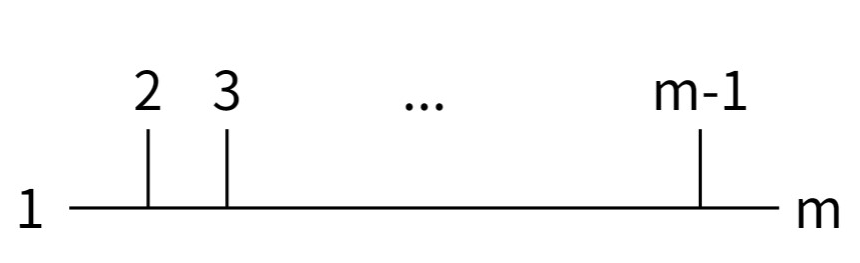
\includegraphics[width=0.4\textwidth]{hl.png}
    \caption{A tree-level $m$-point half-ladder diagram.}
\end{figure}
Using the simplified Feynman rules \eqref{sd-f}, one can derive a general expression for the tree-level numerator of $m$-point diagrams in a half-ladder topology \cite{He:2015wgf}, see figure 1,
\begin{equation}\label{hl}
    n^{\text{s.d.}}_{1|2\cdots (m-1)|m}=(-1)^m\braket{\eta r}^4\left(\prod_{i=1}^m\frac{1}{\langle\eta i\rangle^2}\right)\prod_{j=2}^{m-1}X_{1+2+\cdots+(j-1),j},
\end{equation}
here we do not explicitly label the helicities of the particles, but use $r$ to represent the index associated with the negative helicity state.\par
One can see the vanishing of partial amplitudes by summing over color-ordered diagrams. In this approach, the cancellation is shown by direct computation.
For example,
\begin{equation}
    A^{\text{s.d.}}_4(1,2,4,3)=\frac{n^{\text{s.d.}}_{1|32|4}}{s_{13}}+\frac{n^{\text{s.d.}}_{1|23|4}}{s_{12}}=0,
\end{equation}
and
\begin{equation}
    A^{\text{s.d.}}_5(1,2,3,4,5)=\frac{n^{\text{s.d.}}_{1|234|5}}{s_{12} s_{123}}+(\text{cyc.})=0,
\end{equation}
where $(\text{cyc.})$ means other four terms got by cyclic permutation.
The details of computation are intricate, presented in the appendix \ref{SDYM}.\par
The above calculation serves as a demonstration of the convenience and power of the spinor-helicity formalism. 
However, the main focus of this subsection is to analyze how the kinematic numerators \eqref{hl} exhibit the structure of color-kinematic duality. \par 
Each kinematic numerator is associated with a graph whose color factor $c_i$ takes the form $c_i=f^{abc}\cdots$, 
where the identities among different $c_i$ arise from the antisymmetry and Jacobi identities of the Lie algebra structure constants. 
Remarkably, in the SDYM, the kinematic numerators \eqref{hl} can be constructed in a similar fashion, using coefficients that mirrors the antisymmetry and Jacobi relations of the color factor \cite{Monteiro:2011pc}.
This parallel structure makes the CK duality manifest in this simplified setting. Now we review this construction \cite{Monteiro:2011pc}.\par
We define
\begin{equation}
    {F_{k_1k_2}}^{q}\equiv X_{k_1,k_2}\delta(k_1+k_2-q),
\end{equation}
where $X_{k_1,k_2}$ is defined as the same as the $X_{1,2}$ before and $\delta(k)$ is the Dirac delta function. 
We can using $\delta^{pq}=\delta_{pq}\equiv\delta(p+q)$ raising and lowering indices as,
\begin{equation}
    {F_{k_1k_2q}}=\delta_{qp}{F_{k_1k_2}}^{p}=\int\mathrm{d}^4p \delta(p+q){F_{k_1k_2}}^{p}.
\end{equation}
The contraction of indices is defined as the integral,
\begin{equation}\label{F-contr}
    \begin{split}
        {F_{k_1k_2}}^q {F_{q k_3}}^{p}\equiv& \int \mathrm{d}q X_{k_1,k_2}\delta(k_1+k_2-q)X_{q,k_3}\delta(q+k_3-p)\\
    =&X_{k_1,k_2}X_{k_1+k_2,k_3}\delta(k_1+k_2+k_3-p).
    \end{split}
\end{equation}
We can easily see the antisymmetry of $F^{k_1 k_2 k_3}$ by the definition,
\begin{equation}
    F^{k_1 k_2 k_3}=X_{-k_1,k_1+k_3}\delta(k_1+k_2+k_3)=-X_{-k_1,-k_3}\delta(k_1+k_2+k_3)=F^{k_1k_3k_2}.
\end{equation} 
And the kinematic Jacobi identities,
\begin{equation}
    {F_{k_1 k_2}}^q{F_{qk_3}}^{p}+{F_{k_2 k_3}}^q{F_{qk_1}}^{p}+{F_{k_3 k_1}}^q{F_{qk_2}}^{p}=0,
\end{equation}
which is the consequence of \eqref{X-relation}, mirroring the Lie algebra Jacobi identities,
\begin{equation}
    f^{a_1a_2b}f^{ba_3d}+f^{a_2a_3b}f^{ba_1d}+f^{a_3a_1b}f^{ba_2d}=0.
\end{equation}
In self-dual Yang-Mills theory, only three-point vertices appear, and each vertex is associated simultaneously with a structure constant $f^{abc}$ and a factor $F_{pqk}$. 
These two objects always appear together, so for any given diagram, the color factor and the kinematic numerator naturally exhibit the same algebraic structure. 
However, since the contraction \eqref{F-contr} of the indices of $F_{pqk}$ is somewhat nontrivial, 
we explicitly compute how the tree-level half-ladder numerator \eqref{hl} can be written in terms of the $F$. 
Although this specific numerator vanishes, it still provides a useful illustration of how the kinematic algebra works.\par
The color factor for the half-ladder diagram is,
\begin{equation}
    c_{1|2\cdots(m-1)|m}=f^{a_1a_2 b_1}f^{b_1a_3b_2}\cdots f^{b_{m-3}a_{m-1}a_{m}}.
\end{equation}
By mirroring this, we compute
\begin{equation}
    \begin{split}
    &{F_{k_1k_2}}^{q_1}{F_{q_1k_3}}^{q_2}\cdots {F_{q_{m-4}k_{m-2}}}^{q_{m-3}}{F_{q_{m-3}k_{m-1}k_m}}\\
    =&\int \mathrm{d}q_1\mathrm{d}q_2\cdots \mathrm{d}q_{m-3}X_{k_1,k_2}\delta(k_1+k_2-q_1)X_{q_1,k_3}\delta(q_1+k_3-q_2)\\
    &\qquad\times \cdots \times\delta(q_{m-4}+k_{m-2}-q_{m-3})X_{q_{m-3},k_{m-1}}\delta(q_{m-3}+k_{m-1}+k_m)\\
    =&X_{1,2}X_{1+2,3}\cdots X_{1+\cdots+(m-3),m-2}X_{1+\cdots+(m-2),m-1}\delta(k_1+k_2+\cdots +k_m)\\
    =&\prod_{j=2}^{m-1}X_{1+2+\cdots+(j-1),j}\delta(k_1+k_2+\cdots +k_m).
    \end{split}
\end{equation}
Comparing this result with the numerator \eqref{hl}, we find that they are proportional. Omitting the momentum conservation delta function, 
which is conventionally not included in the definition of the numerators, the expression for the numerator in terms of $F$ reads,
\begin{equation}
    n^{\text{s.d.}}_{1|2\cdots (m-1)|m}=(-1)^m\braket{\eta r}^4\left(\prod_{i=1}^m\frac{1}{\langle\eta i\rangle^2}\right){F_{k_1k_2}}^{q_1}{F_{q_1k_3}}^{q_2}\cdots {F_{q_{m-4}k_{m-2}}}^{q_{m-3}}{F_{q_{m-3}k_{m-1}k_m}}.
\end{equation}
This result naturally exhibits the structure of CK duality.

\subsection{NLSM}
The fact that Born-Infeld (BI) theory can be viewed as the double copy of NLSM and YM theory is revealed through the CHY representation \cite{Cachazo:2014xea,Cachazo:2015ksa}. 
While we will not delve into the technical details of the CHY formalism \cite{Cachazo:2013hca,Cachazo:2013iea}, it is sufficient to note that it encodes double copy structures in a variety of theories, including BI.\par
Motivated by this, we are naturally led to consider possible KLT and BCJ representations for the BI amplitudes. 
The KLT construction will be the focus of the next section. As for BCJ, which stems from color-kinematics duality, 
one is led to ask whether the NLSM amplitudes can be cast into a representation of the form \eqref{acn}. (More precisely, this is a flavor-kinematic duality rather than color-kinematic duality, as the NSLM does not possess color factors.)  
Such constructions have been partially realized in the literature \cite{Du:2016tbc,Carrasco:2016ldy,Carrasco:2016ygv}, and we briefly review them here.\par
The D-dimensional NLSM Lagrangian in the Cayley parametrization is given by \cite{Carrasco:2016ldy},
\begin{equation}
    \mathcal{L}_{\text{NLSM}}=\frac{1}{2}\Tr\left\{\partial_\mu\phi\frac{1}{1-\phi^2}\partial^{\mu}\phi\frac{1}{1-\phi^2}\right\},
\end{equation}
with Lorentz indices $\mu=0,1,\dots, D-1$ and $\phi$ is the Lie-algebra valued Goldstone-boson field.  
This Lagrangian contains infinite number of even-point interaction vertices, making its scattering amplitudes computation nontrivial. And there is no simple way to assign 
numerators to Feynman diagrams using standard Feynman rules. 
The amplitudes can be constructed effeciently using Berends-Giele (BG) \cite{Berends:1987me} recursion relation \cite{Kampf:2012fn}. 
There recursion techniques can be extended to construct a set of a master numerators that reproduce the NLSM amplitudes \cite{Du:2016tbc}. 
The numerators are written as some sum over specific permuted entries of the momentum kernel \eqref{S-kernel}.
% The result of this construction takes the form,
% \begin{equation}
%     n_{1|23\cdots m-1|m}=\sum_{\sigma} S[n-1\cdots 2|\sigma]_1
% \end{equation}
% where $S[\cdot|\cdot]_1$ is the momentum kernel \eqref{S-kernel} and $\sigma$ denotes permutations of $2,3,\dots, n-1$ satisfying specific conditions, see \cite{Du:2016tbc} for details. 
This result later was simplified in \cite{Carrasco:2016ldy}. CK-duality-satisfying $m=2k$ point master numerators are,
\begin{equation}\label{m-num}
    n_{1|\rho(23\cdots 2k-1)|2k}=(-1)^{k}S[\rho(23\cdots 2k-1)|\rho(23\cdots 2k-1)]_1.
\end{equation}
These are referred to as master numerators because the remaining numerators can be determined by imposing the required antisymmetry and kinematic Jacobi identities.
We write four-pint and six-point case explicitly,
\begin{align}
n_{1|23|4}=&s_{12}(s_{13}+s_{23}) \\
n_{1|2345|6}=&-s_{12}(s_{13}+s_{23})(s_{14}+s_{24}+s_{34})(s_{15}+s_{25}+s_{35}+s_{45}).
\end{align}
And the connection between partial NLSM amplitudes and master numerators \eqref{m-num} are,
\begin{equation}\label{A-NLSM}
    A_{2k}^{\text{NLSM}}(\sigma(1,2,\dots,2k-1),2k)=\sum_{\rho\in S_{2k-2}}m[\sigma(12\cdots 2k-1)2k|1\rho(23\cdots 2k-1)2k]n_{1|\rho(23\cdots 2k-1)|2k},
\end{equation}
where $\sigma$ is some permutation of $1,2,\dots,2k-1$ and $m[\cdot|\cdot]$ is the double-partial amplitudes of bi-adjoint scalars \cite{Cachazo:2013iea},
which can be computed as \cite{Mafra:2016ltu},
\begin{equation}
    m[X,n|Y,n]=s_{X}\phi_{X|Y},
\end{equation}
where $X$ and $Y$ are two lists of $1$ to $n-1$ and $\phi_{X|Y}$ is the Berends-Giele double-currents, given recursively by,
\begin{equation}
    \phi_{X|Y}=\frac{1}{s_{X}}\sum_{PQ=X}\sum_{RS=Y}\big(\phi_{P|R}\phi_{Q|S}-(P\leftrightarrow Q)\big),\quad \phi_{i|j}=\delta_{ij},\quad \phi_{X|Y}\equiv 0,\text{ if }X\backslash Y\neq\emptyset.
\end{equation}
Here we compute the four-point examples as a simple check of that the equation \eqref{A-NLSM} correctly reproduces the color-ordered amplitudes of the NLSM.
\begin{equation}
    \begin{split}
    A_4^{\text{NLSM}}(1,2,3,4)=&A_4^{\text{NLSM}}(3,2,1,4)\\
    =&m[1234|1234]n_{1|23|4}+m[1234|1324]n_{1|32|4}\\
    =&\phi_{123|123}S[23|23]_1+\phi_{123|132}S[23|32]_1\\
    =&\Big(\frac{1}{s_{12}}+\frac{1}{s_{23}}\Big)(s_{13}+s_{23})s_{12}+\frac{-1}{s_{23}}(s_{12}+s_{23})s_{13}\\
    =&s_{12}+s_{23},
    \end{split}
\end{equation}
and by the same way,
\begin{equation}
    \begin{split}
    A_4^{\text{NLSM}}(1,3,2,4)=&A_4^{\text{NLSM}}(2,3,1,4)\\
    =&m[1324|1234]n_{1|23|4}+m[1324|1324]n_{1|32|4}\\
    =&s_{13}+s_{23},
    \end{split}
\end{equation}
\begin{equation}
    A_4^{\text{NLSM}}(2,1,3,4)=A_4^{\text{NLSM}}(3,1,2,4)=s_{12}+s_{13},
\end{equation}
which are the same as the results given by another method \cite{Carrasco:2016ldy}. 
And we also present the six-point example \cite{Carrasco:2016ldy}, 
\begin{equation}
    A_6^{\text{NLSM}}(1,2,\dots,6)=s_{12}-\frac{1}{2}\frac{(s_{12}+s_{23})(s_{45}+s_{56})}{s_{123}}+\text{cyclic}(1,2,3,4,5,6).
\end{equation}
%%%%%%%%%%%%%%%%
\section{BI as double copy of YM and NLSM}
In this section, we introduce the BI theory as a double copy of YM and NLSM in the KLT framework. That is,
\begin{equation}\label{4-1}
    \begin{split}
    \mathcal{M}^{\text{BI}}_m(1,2,\dots,m)=&\\
    -i\sum_{\rho ,\sigma\in S_{m-3}}A_m^{\text{NLSM}}&(1,\rho(2,\dots,m-2),m-1,m)S[\rho|\sigma]_1 A_m^{\text{YM}}(1,\sigma(2,\dots,m-2),m,m-1).
    \end{split}
\end{equation}
We do not specify the helicities of external states here, as long as they are consistently assigned in the subsequent calculations.\par
Before delving into the explicit construction of BI amplitudes from this perspective, we first provide a brief 
overview of the BI theory itself and the notable selection rules of its scattering amplitudes.

\subsection{BI theory and selection rule}
Born-Infeld (BI) theory is a nonlinear model of electrodynamics originally proposed by Born and Infeld in 1930s \cite{Born:1934gh}. 
Its Lagrangian takes the form,
\begin{equation}
    \mathcal{L}_{\text{BI}}=\ell^{-2}\left(\sqrt{-\det(\eta_{\mu \nu}-\ell^2 F_{\mu \nu})}-1\right),
\end{equation}
where $\ell$ is the coupling constant. This Lagrangian reduces to Maxwell theory in the weak field limit $F_{\mu \nu}\ll \ell^{-1}$.\par
From this Lagrangian, it is evident that only scattering processes involving an even number of particles can be nonzero. 
This is also natural from the perspective of double copy, since NLSM amplitudes vanish for any odd number of external legs, and according the equation \eqref{4-1},
the BI amplitude inherits this vanishing behavior.\par
A nontrivial selection rule of BI amplitudes states that only helicity configurations with equal numbers of positive and negative helicity photons yield nonvanishing results.
While this can be realized from the structure of BI theory itself \cite{Boels:2008fc}, how this property arise from the KLT double copy remains unclear. 
We will take a brief look at this question in the next subsection.



\subsection{Four-point and six-point tree-level cases}
We begin by presenting the four-dimensional tree-level BI amplitudes in spinor-helicity language \cite{Boels:2008fc} at four points,
\begin{equation}\label{BI-4}
    \mathcal{M}^{\text{BI}}_4(1^-,2^-,3^+,4^+)=-i\braket{12}^2[34]^2,
\end{equation}
\begin{equation}\label{4-zero}
    \mathcal{M}^{\text{BI}}_4(++++)=\mathcal{M}^{\text{BI}}_4(+++-)=\mathcal{M}^{\text{BI}}_4(+---)=\mathcal{M}^{\text{BI}}_4(----)=0,
\end{equation}
and at six-point MHV,
\begin{equation}\label{6-zero}
    \mathcal{M}^{\text{BI}}_6(1^-,2^-,3^+,4^+,5^+,6^+)=0.
\end{equation}
At four points, the YM amplitudes are vanishing except the MHV configuration. 
Through the double copy construction \eqref{4-1}, this directly leads to the results \eqref{4-zero}.
And the four-point MHV amplitude needs a short computation,
\begin{equation}
    \begin{split}
    \mathcal{M}^{\text{BI}}_4(1^-,2^-,3^+,4^+)
    =&-i A_4^{\text{NLSM}}(1,2,3,4)S[2|2]_1 A_4^{\text{YM}}(1^-,2^-,4^+,3^+)\\
    =&i s_{13}s_{12}\frac{\braket{12}^4}{\braket{12}\braket{24}\braket{43}\braket{31}}\\
    =&i\frac{\braket{12}^4 [21][13]}{\braket{24}\braket{43}}\\
    =&i\frac{\braket{12}^2 \braket{43}^2[34]^2[13]}{\braket{24}\braket{43}[21]}\\
    =&i\frac{\braket{12}^2 \braket{43}[34]^2[13]}{\braket{24}[21]}\\
    =&-i\braket{12}^2[34]^2,
    \end{split}
\end{equation}
where $\braket{12}[21]=s_{12}=s_{34}=\braket{43}[34]$ is used in the fourth line and $[13]\braket{34}=\sda{1}{k_3}{4}=-\sda{1}{k_1+k_2+k_4}{4}=[21]\braket{24}$
is used in the last line. This result is indeed \eqref{BI-4}.\par
The six-point case \eqref{6-zero} is considerably more complex. The first nontrivial vanishing amplitude appears at six points in the MHV configuration. 
In this case, both the Yang-Mills and NLSM amplitudes are nonzero, but the KLT double copy gives a vanishing BI amplitudes,
\begin{equation}
    \begin{split}
    \mathcal{M}^{\text{BI}}_6(1^-2^-3^+4^+5^+6^+)=-i\sum_{\rho, \sigma\in S_3}A_6^{\text{NLSM}}(1\rho(234)56)S[\rho|\sigma]_1 A_6^{\text{YM}}(1^-\sigma(2^-3^+4^+)6^+5^+).
    \end{split}
\end{equation}
where the sum runs over $3!\times 3!=36$ terms. In the actual computation, we find that this cancellation does not follow from any simple paring or symmetry.\par
Although the helicity selection rules of BI theory are known, this cancellation illustrates an important point. 
If we could identify a mechanism in the double copy framework that explains why certain amplitudes vanish, such mechanism could potentially be generalized to other theories,
revealing new and previously unknown selection rules for amplitudes.




%%%%%%%%%%%%%%
\section{Conclusion and further directions}
In this report, we have reviewed the double copy structure of scattering amplitudes, revisited how the kinematic algebra can be constructed in SDYM,
and used it to understand the CK duality. We then discussed how the KLT double copy can show the helicity selection rules of BI theory. These examples 
illustrate that double copy is not merely a computational tool, it also reveals deeper symmetries, algebraic structures and constraints in the theories.
There remain many directions for future development and open problems. For instance, how can we construct a kinematic algebra in theories beyond SDYM? 
And how might we understand selection rules at loop-level, or their extensions to other theories, from the double copy perspective.
%%%
\appendix
%%%

\section{Partial amplitudes in SDYM}\label{SDYM}
In this appendix, we directly check the vanishing of SDYM partial amplitudes at four and five points by summing over corresponding numerators.\par
At $m=4$, 
\begin{equation}
    \begin{split}
    A^{\text{tree, s.d.}}_4(1,2,4,3)=&\frac{n^{\text{tree, s.d.}}_{1|32|4}}{s_{13}}+\frac{n^{\text{tree, s.d.}}_{1|23|4}}{s_{12}}\\
    =&C_4\times\bigg(\frac{X_{1,3}X_{1+3,2}}{s_{13}}+\frac{X_{1,2}X_{1+2,3}}{s_{12}}\bigg)\\
    =&C_4\times\bigg(\frac{X_{1,3}X_{1,2}+X_{1,3}X_{3,2}}{s_{13}}+\frac{X_{1,2}X_{1,3}+X_{1,2}X_{2,3}}{s_{12}}\bigg)\\
    =&C_4\times\bigg(-\frac{X_{1,2}X_{1,3}s_{23}}{s_{12}s_{13}}+X_{2,3}\frac{X_{1,2}s_{13}-X_{1,3}s_{12}}{s_{12}s_{13}}\bigg)\\
    =&\frac{C_4}{s_{12}s_{13}}\times\bigg[\braket{1\eta }[12]\braket{2\eta}\braket{\eta 1}[13]\braket{3\eta}\braket{23}[32]+
    \braket{\eta 2}[23]\braket{3\eta}\braket{\eta 1}[12][13]\\
    &\qquad\times\Big(\braket{2\eta}\braket{31}-\braket{3\eta}\braket{21}\Big)\bigg]\\
    =&\frac{C_4}{s_{12}s_{13}}\times \braket{1\eta}\braket{2\eta}\braket{3\eta}[12][13][23]\bigg(\braket{\eta 1}\braket{32}+\braket{\eta 2}\braket{13}+\braket{\eta 3}\braket{21}\bigg)\\
    =&0,
    \end{split}
\end{equation}
where $C_4$ represents the common factor,
\begin{equation*}
    C_4=(-1)^4\braket{\eta r}^4\prod_{i=1}^4\frac{1}{\braket{\eta i}^2}
\end{equation*} and the Schouten identity \eqref{Schouten-a} is used in the final step.\par
At $m=5$,
\begin{equation}\label{a5-s1}
    \begin{split}
    A^{\text{tree, s.d.}}_5(1,2,3,4,5)=&\frac{n^{\text{tree, s.d.}}_{1|234|5}}{s_{12} s_{123}}+(\text{cyc.})\\
    =&C_5\times\frac{X_{1,2}X_{1+2,3}X_{1+2+3,4}}{s_{12}s_{123}}+(\text{cyc.})\\
    =&C_5\times\frac{X_{1,2}X_{1+2,3}X_{4,5}}{s_{12}s_{45}}+(\text{cyc.})\\
    =&\frac{C_5}{2}\Bigg(\frac{X_{1,2}X_{1+2,3}X_{4,5}}{s_{12}s_{45}}-\frac{X_{1,2}X_{4+5,3}X_{4,5}}{s_{12}s_{45}}\Bigg)+(\text{cyc.})\\
    =&\frac{C_5}{2}\Bigg(\frac{X_{1,2}X_{1+2,3}X_{4,5}}{s_{12}s_{45}}-\frac{X_{4,5}X_{2+3,1}X_{2,3}}{s_{45}s_{23}}\Bigg)+(\text{cyc.})
    \end{split}
\end{equation}
In the fourth line, we divide one term into two equal halves and $X_{1+2,3}=-X_{3+4+5,3}=-X_{4+5,3}$ is used. The minus term in the last line comes from the $(\text{cyc.})$ term in the fourth line.
And $C_5$ is the common factor,
\begin{equation*}
    C_5=(-1)^5\braket{\eta r}^4\prod_{i=1}^5\frac{1}{\braket{\eta i}^2}
\end{equation*} Now we begin to prove a useful lemma,
\begin{equation}\label{lemma1}
    \frac{X_{i,j}X_{i+j,l}}{s_{ij}}-\frac{X_{j,l}X_{j+l,i}}{s_{jl}}=\frac{X_{i,j}X_{j,l}s_{ijl}}{s_{ij}s_{jl}}.
\end{equation}
\textbf{Proof.}
\begin{equation*}
    \begin{split}
        &\frac{X_{i,j}X_{i+j,l}}{s_{ij}}-\frac{X_{j,l}X_{j+l,i}}{s_{jl}}\\
        =&X_{i,j}X_{j,l}\frac{s_{ij}+s_{jl}}{s_{ij}s_{jl}}+X_{i,l}\frac{X_{i,j}s_{jl}+X_{j,l}s_{ij}}{s_{ij}s_{jl}}\\
        =&X_{i,j}X_{j,l}\frac{s_{ij}+s_{jl}}{s_{ij}s_{jl}}
        +\Xij{i}{l}\frac{\Xij{i}{j}\braket{jl}[lj]+\Xij{j}{l}\braket{ij}[ji]}{s_{ij}s_{jl}}\\
        =&X_{i,j}X_{j,l}\frac{s_{ij}+s_{jl}}{s_{ij}s_{jl}}
        +\frac{\Xij{i}{l}\braket{j \eta}[lj][ij]\braket{\eta j }\braket{il}}{s_{ij}s_{jl}}\\
        =&X_{i,j}X_{j,l}\frac{s_{ij}+s_{jl}}{s_{ij}s_{jl}}
        +\frac{X_{i,j}X_{j,l}s_{il}}{s_{ij}s_{jl}}\\
        =&\frac{X_{i,j}X_{j,l}s_{ijl}}{s_{ij}s_{jl}},
    \end{split}
\end{equation*}
From the third line to the fourth line, the Schouten identity,
\begin{equation*}
    \braket{\eta i}\braket{jl}+\braket{\eta l}\braket{ij}=\braket{\eta j}\braket{il},
\end{equation*}
is used. By using \eqref{lemma1}, the amplitude \eqref{a5-s1} can be transformed to,
\begin{equation}
    \begin{split}
    A_5^{\text{tree, s.d.}}(1,2,3,4,5)=&\frac{C_5}{2}\frac{X_{1,2}X_{2,3}X_{4,5}}{s_{12}s_{23}}+(\text{cyc.})\\
    =&\frac{C_5}{2}\frac{\etal{1}\etal{2}\etal{3}\etal{4}\etal{5}}{\braket{12}\braket{23}\braket{34}\braket{45}\braket{51}}
        \times{s_{45}\etal{2}\braket{34}\braket{51}}+(\text{cyc.})\\
        \propto& {s_{45}\etal{2}\braket{34}\braket{51}}+(\text{cyc.}),
    \end{split}
\end{equation}
in the last line, the cyclic symmetry of term $\frac{C_5}{2}\frac{\etal{1}\etal{2}\etal{3}\etal{4}\etal{5}}{\braket{12}\braket{23}\braket{34}\braket{45}\braket{51}}$ is used.
This result can be proved to vanish simply by using the Schouten identity \eqref{Schouten-a} and the momentum conservation.
\bibliographystyle{JHEP}
\bibliography{ref}
\end{document}